\documentclass{article}

\usepackage{tipa}			% for \textipa{} macro, displays IPA phonetic notation
\usepackage[bottom]{footmisc}	% footnotes at the bottom of the page

\usepackage{times}
\usepackage{array}		% advanced {array} env manipulations
\usepackage[nodayofweek,level]{datetime} % for date/time formatting
\usepackage{listings}		% synthax highlighting
\usepackage{indentfirst} 		% lightweight package that forces first paragraph after section to have indentation

%\usepackage{layout}		% this package can show the layout parameters of pages
%\usepackage{fancyhdr}		% this package is a flexible way of formatting headers, footers, etc.

\usepackage{multicol}		% used for multi-column layout section

\usepackage{amsmath}		% these packages are for e.g. volume, surface integral signs
\usepackage{amssymb}		% also, amsmath is used for envs that replace inconsistent eqnarray env

\usepackage{graphicx}		% to insert images/figures
\usepackage{subcaption}		% to insert subfigures - images next to each other in a row
\usepackage{floatrow}		% for limiting the caption width

% folder where images that will be displayed in figures are located
\graphicspath{ {img/} }

% page layout (size, margins, etc.) setup
\usepackage{geometry}
\geometry
{
a4paper,
margin=1.5in
}

% these packages are for pseudocode formatting
\usepackage{algorithm,algorithmicx,algpseudocode}

% package which redefines bibliography section to contain number and be reflected in ToC
\usepackage{etoolbox}
\patchcmd{\thebibliography}{*}{}{}{}

% this package doesn't work with pdfLaTeX, well fine, I didn't want it anyway, meeh
%\usepackage{unicode-math}	% additional symbols (like \Omicron)

% this macro allows to number specific lines for {align*} env
\newcommand\numberthis{\addtocounter{equation}{1}\tag{\theequation}}

\newdate{cheatsheet_date}{10}{7}{2017}

%\usepackage{commath}	
% this package has useful shortcuts for math: \od OR \od[2] - fractional derivative

% These defines needed for upright integral symbol
% BEGIN - UPRIGHT INT

\DeclareFontFamily{U}{mathx}{\hyphenchar\font45}
\DeclareFontShape{U}{mathx}{m}{n}{<->mathx10}{}
\DeclareFontSubstitution{U}{mathx}{m}{n}
\DeclareSymbolFont{mathx}{U}{mathx}{m}{n}

% These define new operator, \vint* - but could also be used to redefine standard operators, see the '\ifuprightint' code below
\DeclareMathSymbol{\vint}   {\mathop}{mathx}{"B3}
\DeclareMathSymbol{\viint}  {\mathop}{mathx}{"B4}
\DeclareMathSymbol{\viiint} {\mathop}{mathx}{"B5}
\DeclareMathSymbol{\voint} {\mathop}{mathx}{"B6}
\DeclareMathSymbol{\voiint}{\mathop}{mathx}{"B7}

\newif\ifuprightint

% Uncomment if you want upright integrals by default
%\uprightinttrue
\ifuprightint

\DeclareMathSymbol{\intop}   {\mathop}{mathx}{"B3}
\DeclareMathSymbol{\iintop}  {\mathop}{mathx}{"B4}
\DeclareMathSymbol{\iiintop} {\mathop}{mathx}{"B5}
\DeclareMathSymbol{\ointop} {\mathop}{mathx}{"B6}
\DeclareMathSymbol{\oiintop}{\mathop}{mathx}{"B7}

\fi

% END - UPRIGHT INT

\newcommand*\diff{\mathop{}\!\mathrm{d}}
\newcommand*\diffe[1]{\mathop{}\!\mathrm{d^#1}}
\newcommand*\tr{\mathop{}\!\mathrm{tr}}

% replace this in order to get different designation for higher limits
\newcommand*\hlim{\mathop{}\! h}
%\newcommand*\hlim{\mathop{}\! \hslash}

% commands for enhanced control over algorithmic indentation
\algdef{se}[MyBlock]{IndentBlock}{EndIndentBlock}	% defining custom block
\algtext*{IndentBlock}					% force remove line for the block start
\algtext*{EndIndentBlock}				% force remove line for the block end

% Setting up how section titles will look
\usepackage{titlesec}
\titlelabel{\thetitle.\quad}

\begin{document}

% The empty braces "{}" are required for macro here for parser not to consume spaces
\title{\LaTeX{} cheatsheet: a collection of useful \LaTeX{} examples}
\author{
Andrey Voroshilov,\\
Moscow
}
\date{\displaydate{cheatsheet_date}}
\maketitle

\begin{abstract}
This example shows several useful examples of how to use \LaTeX{} and some of the additional packages to format/reference formulae, algorithms and images.
\end{abstract}

\thispagestyle{empty}		% this command sets style for headers & footers for the current page only (blank)

% \section* means unnumbered section - this section should be not listed in ToC
\section*{Introduction}
\LaTeX{} is a document preparation system. Pronounced \textipa{/'lA:tEx/}.\\

It is widely used in academia publications, and with packages like MathJax - to display formulae on websites. \\

This document is intended to show how to design basic elements of a \LaTeX{} document, as solving some of the common issues without prior knowledge might become painful.\\

\newpage

\tableofcontents

\newpage

\section{Section}

\subsection{Basic text} \label{sec:basic_text}
Some inline text styles: \textbf{bold}, \textit{italic}, \textrm{roman (serif)}, \textsf{sans-serif}, \textnormal{forced "normal" text}. Within math environments, it is recommended to use "normal" text, contrary to the common usage of "roman (serif)" macro: in case general document font will change to sans-serif (or due to copying between different documents with different font styles), no modification of math envs will be required.
\begin{center}
Spacing symbols:\\
\begin{tabular} {l | l}
\hline
\textbackslash! & hello\!space \\
\textbackslash, & hello\,space \\
\textbackslash: & hello\:space \\
\textbackslash; & hello\;space \\
\textbackslash quad & hello{\quad}space  \\
\textbackslash qquad & hello{\qquad}space  \\
\hline
\end{tabular}
\end{center}

\begin{center}
Accent  symbols:\\
\begin{tabular} {c | c | c | c }
{\LaTeX} \textbf{text} & example & {\LaTeX} \textbf{math} & example \\
\hline
\textbackslash` & \`a & \textbackslash grave  & $\grave{a}$ \\
\textbackslash' & \'a & \textbackslash acute & $\acute{a}$ \\
\textbackslash\textasciicircum & \^a & \textbackslash hat & $\hat{a}$ $\hat{\imath}$ \\
 &  & \textbackslash widehat & $\widehat{aa}$ \\
\textbackslash" & \"a \"{\i} & \textbackslash ddot & $\ddot{a}$ \\
\textbackslash\~ & \~a & \textbackslash tilde & $\tilde{a}$ \\
 &  & \textbackslash widetilde & $\widetilde{aa}$ \\
\textbackslash H & \H a & & \\
\textbackslash c & \c a & & \\
\textbackslash = & \={a} \={\j} & \textbackslash bar & $\bar{a}$ $\bar{\jmath}$ \\
 &  & \textbackslash vec & $\vec{a}$ $\vec{\imath}$ \\
\textbackslash b & \b{a} & & \\
\textbackslash . & \.{a} & \textbackslash dot & $\dot{a}$ \\
\textbackslash d & \d{a} & & \\
\textbackslash r & \r{a} & & \\
\textbackslash u & \u{a} & \textbackslash breve & $\breve{a}$ \\
\textbackslash v & \v{a} & \textbackslash check & $\check{a}$ \\
\textbackslash t & \t{aa} & & \\

\hline
\end{tabular}
\end{center}

One could reference\footnote{It could require two typesetting runs to propagate referencing changes, on a first run if references were changed, you could see wrong numbers, or even bold question marks (like this: \ref{non_existent})}
subsection like this: see display-style math in \S \ref{sec:complex_math}, equations like this: Equation (\ref{eq:complex_multiline}) and Equation (\ref{eq:complex_multiline_german}), and other works as was proposed by A. Author et al., \cite{author2016}. Pictures/figures could be referenced as well: Figure \ref{fig:style_transfer}, or a certain picture in the whole figure - van Gogh style is present in Figure \ref{fig:style_transfer_a}. Algorithms could be referenced too, for the original version of Euclid's algorithm, see Algorithm \ref{alg:original_euclid}.

And a lists examples:\\
Unordered:
\begin{itemize}
  \item Item1.
  \begin{itemize}
    \item Subitem1.
    \item Subitem2.
    \item Subitem3.
  \end{itemize}
  \item Item2.
  \item Item3.
\end{itemize}
Ordered:
\begin{enumerate}
  \item Item1.
  \item Item2.
  \begin{enumerate}
    \item Subitem1.
    \item Subitem2.
    \item Subitem3.
  \end{enumerate}
  \item Item3. Note how the counter is manually set to some value, resulting in sublist starting with (k).
  \begin{enumerate}
    \setcounter{enumii}{10}
    \item Subitem1.
    \item Subitem2.
    \item Subitem3.
  \end{enumerate}
\end{enumerate}


\subsection{Basic math} \label{sec:basic_math}

\textit{Sed ut perspiciatis, unde omnis iste natus error sit voluptatem accusantium doloremque laudantium, totam rem aperiam eaque ipsa, quae ab illo inventore veritatis et quasi architecto beatae vitae dicta sunt, explicabo.}\\
Here is some text with \textbf{text-math} in it: $\mathbf{x}^{T}\mathbf{x} = \sum_{i=1}^k x_i x_i = |\mathbf{x}|^{2}$.\\
\textit{Nemo enim ipsam voluptatem, quia voluptas sit, aspernatur aut odit aut fugit, sed quia consequuntur magni dolores eos, qui ratione voluptatem sequi nesciunt, neque porro quisquam est, qui dolorem ipsum, quia dolor sit amet consectetur adipisci velit, sed quia non numquam eius modi tempora incidunt, ut labore et dolore magnam aliquam quaerat voluptatem.}\\

And another example of display-math:
$$
\mathbf{x}^{T}\mathbf{x} = \sum_{i=1}^k x_i x_i = |\mathbf{x}|^{2}
$$

\textit{Sed ut perspiciatis, unde omnis iste natus error sit voluptatem accusantium doloremque laudantium, totam rem aperiam eaque ipsa, quae ab illo inventore veritatis et quasi architecto beatae vitae dicta sunt, explicabo.}\\
And additional example of \textbf{display-math} within text: $\displaystyle\mathbf{x}^{T}\mathbf{x} = \sum_{i=1}^k x_i x_i = |\mathbf{x}|^{2}$.\\
\textit{Nemo enim ipsam voluptatem, quia voluptas sit, aspernatur aut odit aut fugit, sed quia consequuntur magni dolores eos, qui ratione voluptatem sequi nesciunt, neque porro quisquam est, qui dolorem ipsum, quia dolor sit amet consectetur adipisci velit, sed quia non numquam eius modi tempora incidunt, ut labore et dolore magnam aliquam quaerat voluptatem.}\\

As it could be seen, this increases row-space.\\
\\
Examples of various differential symbols: $\frac{\diff f(x)}{\diff x}$, $\frac{\partial \mathbf{f}(x, y)}{\partial x}$.\\
\\

Math formula with reference:
\begin{equation} \label{eq:e_mc2}
E_{r}^{2}-|{\vec {p}}\,|^{2}c^{2}=m_{0}^{2}c^{4}
\end{equation}

Math formula without number next to it (it still can be referenced by the label, but it will reference section instead):
\begin{equation*} \label{eq:accents}
\widetilde{[\xi]}
\end{equation*}

% Use amsmath package
You can also write bold math symbols like that: $\boldsymbol{\lambda}$ vs $\lambda$, $\boldsymbol{\Sigma}$ vs $\Sigma$ and so on.\\

To display nested math symbols fractions as display style (full-size), use \textbf{\textbackslash dfrac} from \textit{amsmath}; on the contrary, to show fraction as text-inline size, use \textbf{\textbackslash tfrac}:
$$
\dfrac{1}{2} = \tfrac{1}{2}
$$



\subsection{Complex math and preprocessor} \label{sec:complex_math}

Complex multi-line formula with integrals example, with reference at the final line (notice \textbf{\textbackslash nonumber} on the first line - without it, each line of the equation would be marked with a reference number):
\begin{align} \label{eq:complex_multiline}
\iint \limits _{S}\left(\mathbf{F} \cdot \mathbf{n}\right) \diff S = & \iint \limits _{S}\left(\mathbf{F}_{x} \cos{\alpha} + \mathbf{F}_{y} \cos{\beta} + \mathbf{F}_{z} \cos{\gamma}\right) \diff S \nonumber \\
= & \iiint \limits _{V} \left( \nabla \cdot \mathbf{F} \right) \diff V
\end{align}

Additional thing to notice in this example - is that the integral is upright. There are different styles of the integral symbol, all have different leaning. English-style is leaning to the right (as in the example (\ref{eq:complex_multiline}) above). Russian integral style is leaning to the left. German (or Central European) integral style is upright (as in example (\ref{eq:complex_multiline_german}) below). Check out the source header to see how the upright integrals are defined.

\begin{align} \label{eq:complex_multiline_german}
\viint \limits _{S}\left(\mathbf{F} \cdot \mathbf{n}\right) \diff S = & \viint \limits _{S}\left(\mathbf{F}_{x} \cos{\alpha} + \mathbf{F}_{y} \cos{\beta} + \mathbf{F}_{z} \cos{\gamma}\right) \diff S \nonumber \\
= & \viiint \limits _{V} \left( \nabla \cdot \mathbf{F} \right) \diff V
\end{align}

Matrix example + extra example of preprocessor switches (check out the source code for preprocessor directives \textbf{\textbackslash newif} and \textbf{\textbackslash fi}):
\newif\ifoneformulakind
% Uncomment the line below, to get the intermediate vector view
%\oneformulakindtrue
$$
\textnormal{V}
\ifoneformulakind
= \left[
\begin{array}{c}
\mathbf{v}_{1}^{T} \\
\mathbf{v}_{2}^{T} \\
\mathbf{v}_{3}^{T}
\end{array}
\right]
\fi
= \left[
\begin{array}{c c c}
{\mathbf{v}_{1}}_{x} & {\mathbf{v}_{1}}_{y} & {\mathbf{v}_{1}}_{z} \\
{\mathbf{v}_{2}}_{x} & {\mathbf{v}_{2}}_{y} & {\mathbf{v}_{2}}_{z} \\
{\mathbf{v}_{3}}_{x} & {\mathbf{v}_{3}}_{y} & {\mathbf{v}_{3}}_{z}
\end{array}
\right]
$$

One way to describe the linear system:
\begin{equation} \label{eq:linear_system_example}
\left\{
\begin{array} {r l}
\mathbf{a} + \mathbf{b} & = \mathbf{c} + \mathbf{d} +\mathbf{e} , \\
\mathbf{b} & = -\mathbf{d}
\end{array}
\right.
\end{equation}


\subsection{Algorithms and images} \label{sec:algorithms_images}

% Note [H] - this is a placement hint, meaning the image should be placed where it is defined ("here"). Possible alternatives are e.g. [t], [b], [p], or even no hint at all.
% Image files are searched in locations provided by "\graphicspath" in the header
\begin{figure}[H]
  \centering
  \begin{subfigure}[b]{0.45\linewidth}
    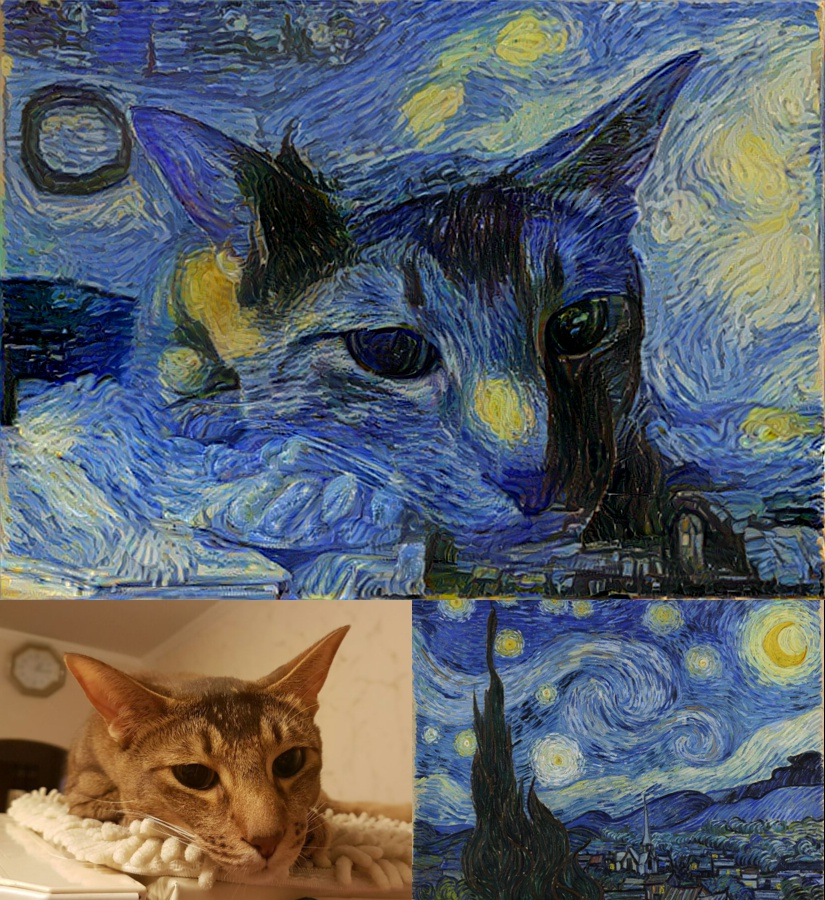
\includegraphics[width=\linewidth]{style_transfer01.jpg}
    \caption{Example of style transfer \label{fig:style_transfer_a}}
  \end{subfigure}
  \begin{subfigure}[b]{0.45\linewidth}
    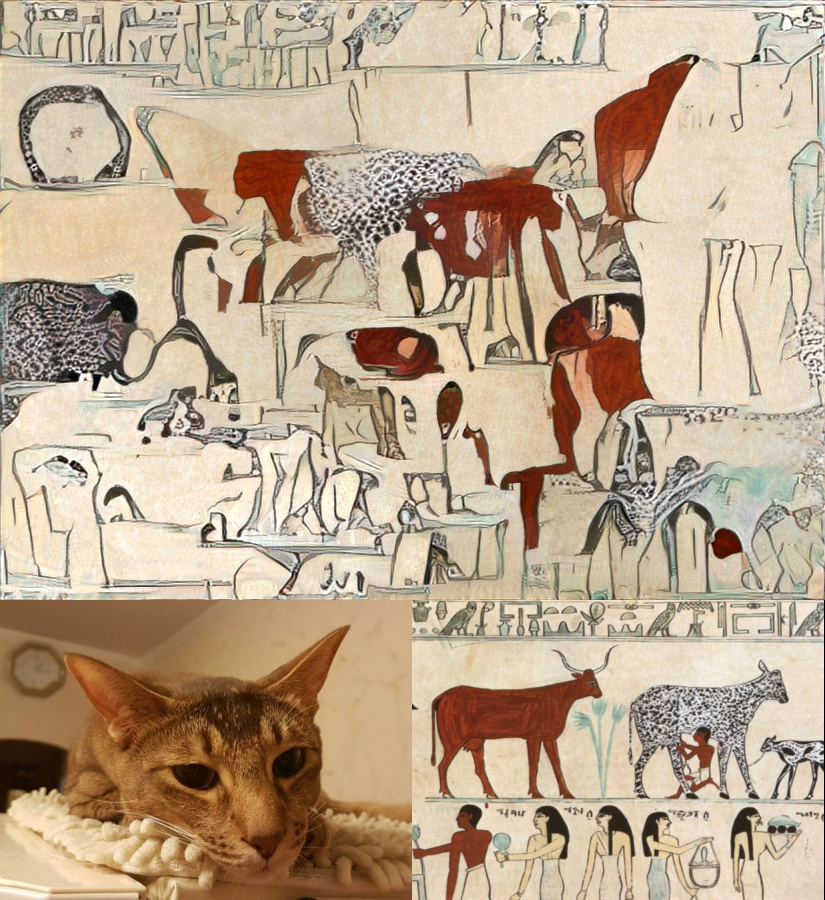
\includegraphics[width=\linewidth]{style_transfer02.jpg}
    \caption{Another example of style transfer \label{fig:style_transfer_b}}
  \end{subfigure}
  \ffigbox[\FBwidth]{
  \caption{Results of optimization-based style transfer \label{fig:style_transfer}}
  }{\rule{30em}{0mm}}
\end{figure}

And here's how algorithms could be typeset: \\

\begin{algorithm}[H]
\caption{The original Euclid's algorithm}
\label{alg:original_euclid}
\begin{algorithmic}[1]
\Require {$a$ and $b$ - positive integers}
\IndentBlock

% Step 0. Initialization
%\State\hspace{-1.8em} {Step 0. {\it \{Initialization\} }}
\Statex {\textit{Function that returns \textnormal{Greatest Common Divisor}}.}
\Statex {\textit{Note how function block has excessive incentation - this is on purpose, to show forced indentation via manual commands \textnormal{\textbf{\textbackslash IndentBlock}} and \textnormal{\textbf{\textbackslash EndIndentBlock}}}.}
    \Function {GCD}{$a$, $b$}
        \While {$a \neq b$}
\Statex {\textit{There is better version that uses $\textnormal{mod}$ operator (remainder calculation)}}
            \If {$a > b$}
                \State {$a = a - b$}
            \Else
                \State {$b = b - a$}
            \EndIf
        \EndWhile
        \State \Return {$a$}
    \EndFunction

 \EndIndentBlock
\end{algorithmic}
\end{algorithm}



\newpage

\begin{thebibliography}{99}

	\bibitem{author2016}
		A. Author,
		\emph{The Book of Knowledge},
		2016

	\bibitem{author2017}
		A. Author,
		\emph{The Book of Additional Knowledge},
		2017

\end{thebibliography}
\end{document}